\subsection{Stress}\label{sec:Str}
Stress in Amarasi falls on the penultimate syllable of the prosodic word.
Usually this means the penultimate segmental vowel is stressed.
The three main correlates of stress in Amarasi are duration, pitch, and intensity.
A stressed vowel is typically realised with higher pitch,
increased intensity, and is longer when compared to unstressed vowels.

A simple example can be seen in the word \ve{nisi-f} {\ra} [ˈnisɪf] {\emb{nisif.mp3}{\spk{}}{\apl}} `tooth'.
The spectrogram for one repetition of this word in a wordlist is given in Figure \ref{fig:SpeNis}.
Intensity is shown by the solid yellow line and pitch by the dotted blue lines.

\begin{figure}[h]
	\centering\setlength\fboxsep{-0.5pt}\setlength\fboxrule{0.75pt}
			\caption{Spectrogram of [ˈnisɪf] `tooth'}
		\fbox{\includegraphics[width=\textwidth]{nisif.eps}}
	\label{fig:SpeNis}
\end{figure}

\begin{table}[ht]
	\centering\caption{Length, pitch, and intensity of vowels in [ˈnisɪf] `tooth'}\label{tab:LenPitIntVowNis}
		\begin{tabular}{rll} \lsptoprule
										& V\sub{1}& V\sub{2} \\ \midrule
			length (sec)	&   0.095	&   0.07 \\ 
			peak intensity (dB)&  80	&  75 \\ 
			peak pitch (Hz)		& 207	& 186 \\ \lspbottomrule
		\end{tabular}
\end{table}

Visually, it is quite clear from Figure \ref{fig:SpeNis} that the initial vowel has higher pitch
as well as increased intensity and duration when compared to the second vowel.
The measurements for length, intensity, and duration for both vowels
in this recording are given in \trf{tab:LenPitIntVowNis}.
These figures can be considered broadly representative of the pattern observed for all feet.

Words with the surface structure VVCV(C){\#}
are the only words in which the penultimate vowel is not stressed.
The initial vowel sequence of such words is usually realised as a phonetic diphthong,
with the higher vowel realised as an off-glide.
The whole phonetic diphthong is then the locus of stress placement.
Examples are given in \qf{ex:(C)VVCV(C)->"(C)VVCV(C)} below.
This otherwise irregular stress is analysed by positing 
that the first two vowels are assigned to a single V-slot (\srf{sec:Syl}).

\begin{exe}
	\ex{(C)VVCV(C) {\ra} ˈ(C)VVCV(C) \label{ex:(C)VVCV(C)->"(C)VVCV(C)}}
		\sn{\gw\begin{tabular}{llll}
			\ve{kaunaʔ}	& [\tbr{ˈ}k\tbr{ɐw}nɐʔ]		&{\emb{kaunaq.mp3}{\spk{}}{\apl}}	& `snake; creature'\\
			\ve{aikaʔ}	& [\tbr{ˈ}ʔ\tbr{aj}kaʔ]		&{\emb{aikaq.mp3}{\spk{}}{\apl}}	& `thorn' \\
			\ve{nautus}	& [\tbr{ˈ}n\tbr{əw}t̪ʊs]&{\emb{nautus.mp3}{\spk{}}{\apl}}	& `beetle' \\
			\ve{naunuʔ}	& [\tbr{ˈ}n\tbr{əw}nʊʔ] 	&{\emb{naunuq.mp3}{\spk{}}{\apl}}	& `breadfruit' \\
			\ve{uaba-ʔ}	& [\tbr{ˈ}ʔ\tbr{wɐ}bɐʔ]		&{\emb{uabaq.mp3}{\spk{}}{\apl}}	& `speech, language' \\
		\end{tabular}}
\end{exe}

For words with more than two syllables,
secondary stress is assigned to every second syllable to the left of the primary stress.
This provides evidence that non-final feet form separate prosodic words.
Two examples are \ve{ataʔraʔe} `praying mantis' {\ra} [\tbr{ˌ}ʔat̪aʔˈraʔɛ]{\emb{ataqraqe.mp3}{\spk{}}{\apl}}
and \ve{ai\j onuus} `kind of herb' [\tbr{ˌ}ʔajʤɔ̝ˈnʊːs]{\emb{aijonuus.mp3}{\spk{}}{\apl}}.
The structures of each of these words are shown in \qf{as:PrWd:ataqraqe}
and \qf{as:PrWd:aijonuus} respectively.
While each of these words contains two prosodic words,
they are single morphemes, as indicated by the \emph{M} on the bottom tier.

%naiso'o
%naiso muti'
%naiso me'e
%naiso no'o

\begin{multicols}{2}
	\begin{exe}
		\exa{\label{as:PrWd:ataqraqe}\xy
				<3em,5cm>*\as{PrWd}="PrWd1",<8em,5cm>*\as{PrWd}="PrWd2",
				<3em,4cm>*\as{Ft}="ft1",<8em,4cm>*\as{Ft}="ft2",
				<2em,3cm>*\as{σ}="s1",<4em,3cm>*\as{σ}="s2",<7em,3cm>*\as{σ}="s3",<9em,3cm>*\as{σ}="s4",
				<1em,2cm>*\as{C}="CV1",<2em,2cm>*\as{V}="CV2",<3em,2cm>*\as{C}="CV3",<4em,2cm>*\as{V}="CV4",<5em,2cm>*\as{C}="CV5",
				<6em,2cm>*\as{C}="CV6",<7em,2cm>*\as{V}="CV7",<8em,2cm>*\as{C}="CV8",<9em,2cm>*\as{V}="CV9",<10em,2cm>*\as{C}="CV10",
				<1em,1cm>*\as{}="cv1",<2em,1cm>*\as{a}="cv2",<3em,1cm>*\as{t}="cv3",<4em,1cm>*\as{a}="cv4",<5em,1cm>*\as{ʔ}="cv5",
				<6em,1cm>*\as{r}="cv6",<7em,1cm>*\as{a}="cv7",<8em,1cm>*\as{ʔ}="cv8",<9em,1cm>*\as{e}="cv9",<10em,1cm>*\as{}="cv10",
				<5.5em,0cm>*\as{M}="m1",
				"m1"+U;"cv2"+D**\dir{-};"m1"+U;"cv3"+D**\dir{-};"m1"+U;"cv4"+D**\dir{-};"m1"+U;"cv5"+D**\dir{-};
				"m1"+U;"cv6"+D**\dir{-};"m1"+U;"cv7"+D**\dir{-};"m1"+U;"cv8"+D**\dir{-};"m1"+U;"cv9"+D**\dir{-};
				"cv2"+U;"CV2"+D**\dir{-};"cv3"+U;"CV3"+D**\dir{-};"cv4"+U;"CV4"+D**\dir{-};"cv5"+U;"CV5"+D**\dir{-};
				"cv6"+U;"CV6"+D**\dir{-};"cv7"+U;"CV7"+D**\dir{-};"cv8"+U;"CV8"+D**\dir{-};"cv9"+U;"CV9"+D**\dir{-};
				"CV1"+U;"s1"+D**\dir{-};"CV2"+U;"s1"+D**\dir{-};"CV3"+U;"s1"+D**\dir{-};
				"CV3"+U;"s2"+D**\dir{-};"CV4"+U;"s2"+D**\dir{-};"CV5"+U;"s2"+D**\dir{-};
				"CV6"+U;"s3"+D**\dir{-};"CV7"+U;"s3"+D**\dir{-};"CV8"+U;"s3"+D**\dir{-};
				"CV8"+U;"s4"+D**\dir{-};"CV9"+U;"s4"+D**\dir{-};"CV10"+U;"s4"+D**\dir{-};
				"s1"+U;"ft1"+D**\dir{-};"s2"+U;"ft1"+D**\dir{-};"s3"+U;"ft2"+D**\dir{-};"s4"+U;"ft2"+D**\dir{-};
				"ft1"+U;"PrWd1"+D**\dir{-};"ft2"+U;"PrWd2"+D**\dir{-};
		\endxy}
		\exa{\label{as:PrWd:aijonuus}\xy
				<3em,5cm>*\as{PrWd}="PrWd1",<8em,5cm>*\as{PrWd}="PrWd2",
				<3em,4cm>*\as{Ft}="ft1",<8em,4cm>*\as{Ft}="ft2",
				<2em,3cm>*\as{σ}="s1",<4em,3cm>*\as{σ}="s2",<7em,3cm>*\as{σ}="s3",<9em,3cm>*\as{σ}="s4",
				<1em,2cm>*\as{C}="CV1",<2em,2cm>*\as{V}="CV2",<3em,2cm>*\as{C}="CV3",<4em,2cm>*\as{V}="CV4",<5em,2cm>*\as{C}="CV5",
				<6em,2cm>*\as{C}="CV6",<7em,2cm>*\as{V}="CV7",<8em,2cm>*\as{C}="CV8",<9em,2cm>*\as{V}="CV9",<10em,2cm>*\as{C}="CV10",
				<1.75em,1cm>*\as{a}="cv1",<2.25em,1cm>*\as{i}="cv2",<3em,1cm>*\as{\j}="cv3",<4em,1cm>*\as{o}="cv4",<5em,1cm>*\as{}="cv5",
				<6em,1cm>*\as{n}="cv6",<7em,1cm>*\as{u}="cv7",<8em,1cm>*\as{}="cv8",<9em,1cm>*\as{u}="cv9",<10em,1cm>*\as{s}="cv10",
				<5.75em,0cm>*\as{M}="m1",
				"m1"+U;"cv1"+D**\dir{-};"m1"+U;"cv2"+D**\dir{-};"m1"+U;"cv3"+D**\dir{-};"m1"+U;"cv4"+D**\dir{-};
				"m1"+U;"cv6"+D**\dir{-};"m1"+U;"cv7"+D**\dir{-};"m1"+U;"cv9"+D**\dir{-};"m1"+U;"cv10"+D**\dir{-};
				"cv1"+U;"CV2"+D**\dir{-};"cv2"+U;"CV2"+D**\dir{-};"cv3"+U;"CV3"+D**\dir{-};"cv4"+U;"CV4"+D**\dir{-};"cv5"+U;"CV5"+D**\dir{};
				"cv6"+U;"CV6"+D**\dir{-};"cv7"+U;"CV7"+D**\dir{-};"cv8"+U;"CV8"+D**\dir{};"cv9"+U;"CV9"+D**\dir{-};"cv10"+U;"CV10"+D**\dir{-};
				"CV1"+U;"s1"+D**\dir{-};"CV2"+U;"s1"+D**\dir{-};"CV3"+U;"s1"+D**\dir{-};
				"CV3"+U;"s2"+D**\dir{-};"CV4"+U;"s2"+D**\dir{-};"CV5"+U;"s2"+D**\dir{-};
				"CV6"+U;"s3"+D**\dir{-};"CV7"+U;"s3"+D**\dir{-};"CV8"+U;"s3"+D**\dir{-};
				"CV8"+U;"s4"+D**\dir{-};"CV9"+U;"s4"+D**\dir{-};"CV10"+U;"s4"+D**\dir{-};
				"s1"+U;"ft1"+D**\dir{-};"s2"+U;"ft1"+D**\dir{-};"s3"+U;"ft2"+D**\dir{-};"s4"+U;"ft2"+D**\dir{-};
				"ft1"+U;"PrWd1"+D**\dir{-};"ft2"+U;"PrWd2"+D**\dir{-};
		\endxy}
	\end{exe}
\end{multicols}

The penultimate vowel of the final nominal of 
the noun phrase bears primary stress
with secondary stress being assigned
to every second syllable to the left.
Examples of noun phrases with this stress pattern
are given in \qf{ex:StrNouNouAdj} below.

\begin{exe}
	\ex{Stress for nominal + nominal:\label{ex:StrNouNouAdj}}
		\sn{\gw\begin{tabular}{rclll}
			\ve{aam babaʔ}	&\ra& [ˌʔamˈbabaʔ]	&{\emb{aam-babaq.mp3}{\spk{}}{\apl}}&`father' + `MB/FZ'\\
			\ve{ain babaʔ}	&\ra& [ˌʔæjnˈbabɐʔ]&{\emb{ain-babaq.mp3}{\spk{}}{\apl}}&`mother' + `MB/FZ'\\
			\ve{hau noʔo}	&\ra& [ˌhawˈnɔʔɔ]			&{\emb{hau-noqo.mp3}{\spk{}}{\apl}}	&`tree' + `leaf'		\\
			\ve{ʔnaak funu-f}	&\ra& [ˌʔnakˈfʊnʊf]			&{\emb{qnaak-funuf.mp3}{\spk{}}{\apl}}	&`head' + `hair'	\\
			\ve{atoin munif}	&\ra& [ʔaˌt̪ɵjnˈmʊnɪf]	&{\emb{atoin-munif.mp3}{\spk{}}{\apl}}&`man' + `young'	\\
			\ve{oe mninuʔ}	&\ra& [ˌʔɔɛmˈninʊʔ]		&{\emb{oe-mninuq.mp3}{\spk{}}{\apl}}	&`water' + `drinkable'\\
			\ve{raan metoʔ}	&\ra& [ˌhɾanˈmɛt̪ɔʔ]	&{\emb{raan-metoq.mp3}{\spk{}}{\apl}}	&`road' + `dry'		\\
			\ve{umi mnasiʔ}	&\ra& [ˌʔʊmimˈnasiʔ]		&{\emb{umi-mnasiq.mp3}{\spk{}}{\apl}}	&`house' + `old'	\\
			\ve{mais{\gap}oni}	&\ra& [ˌmajsˈʔoni]	&{\emb{mais-oni.mp3}{\spk{}}{\apl}}	&`salt' + `sugar'	\\ \hhline{}
				&		&							&																		&(=`crystalline sugar') \\
		\end{tabular}}
\end{exe}

There is no difference in the prosodic structure
of a nominal phrase with multiple nominals
compared with a single word greater than three syllables.
The structures of \ve{raan metoʔ} `dry road'
and \ve{umi mnasiʔ} `old house' are given in \qf{as:PrWd:raan-metoq}
and \qf{as:PrWd:umi-mnasiq} respectively.
In the case of \ve{raan metoʔ} `dry road' the first noun
has undergone metathesis (from \ve{ranan} `road') and thus occurs
with the derived CVVC M-foot (\srf{sec:TheFoo}).

\begin{multicols}{2}
	\begin{exe}
		\exa{\label{as:PrWd:raan-metoq}\xy
				<2.5em,5cm>*\as{PrWd}="PrWd1",<7em,5cm>*\as{PrWd}="PrWd2",
				<2.5em,4cm>*\as{\hp{\sub{\tsc{m}}}Ft\sub{\tsc{m}}}="ft1",<7em,4cm>*\as{Ft}="ft2",
				<1.5em,3cm>*\as{σ}="s1",<3.5em,3cm>*\as{σ}="s2",<6em,3cm>*\as{σ}="s3",<8em,3cm>*\as{σ}="s4",
				<1em,2cm>*\as{C}="CV1",<2em,2cm>*\as{V}="CV2",<3em,2cm>*\as{V}="CV3",<4em,2cm>*\as{C}="CV4",
				<5em,2cm>*\as{C}="CV5",<6em,2cm>*\as{V}="CV6",<7em,2cm>*\as{C}="CV7",<8em,2cm>*\as{V}="CV8",<9em,2cm>*\as{C}="CV9",
				<1em,1cm>*\as{r}="cv1",<2em,1cm>*\as{a}="cv2",<3em,1cm>*\as{a}="cv3",<4em,1cm>*\as{n}="cv4",
				<5em,1cm>*\as{m}="cv5",<6em,1cm>*\as{e}="cv6",<7em,1cm>*\as{t}="cv7",<8em,1cm>*\as{o}="cv8",<9em,1cm>*\as{ʔ}="cv9",
				<2.5em,0cm>*\as{M}="m1",<7em,0cm>*\as{M}="m2",
				"m1"+U;"cv1"+D**\dir{-};"m1"+U;"cv2"+D**\dir{-};"m1"+U;"cv3"+D**\dir{-};"m1"+U;"cv4"+D**\dir{-};
				"m2"+U;"cv5"+D**\dir{-};"m2"+U;"cv6"+D**\dir{-};"m2"+U;"cv7"+D**\dir{-};"m2"+U;"cv8"+D**\dir{-};"m2"+U;"cv9"+D**\dir{-};
				"cv1"+U;"CV1"+D**\dir{-};"cv2"+U;"CV2"+D**\dir{-};"cv3"+U;"CV3"+D**\dir{-};"cv4"+U;"CV4"+D**\dir{-};"cv5"+U;"CV5"+D**\dir{-};
				"cv6"+U;"CV6"+D**\dir{-};"cv7"+U;"CV7"+D**\dir{-};"cv8"+U;"CV8"+D**\dir{-};"cv9"+U;"CV9"+D**\dir{-};
				"CV1"+U;"s1"+D**\dir{-};"CV2"+U;"s1"+D**\dir{-};
				"CV3"+U;"s2"+D**\dir{-};"CV4"+U;"s2"+D**\dir{-};
				"CV5"+U;"s3"+D**\dir{-};"CV6"+U;"s3"+D**\dir{-};"CV7"+U;"s3"+D**\dir{-};
				"CV7"+U;"s4"+D**\dir{-};"CV8"+U;"s4"+D**\dir{-};"CV9"+U;"s4"+D**\dir{-};
				"s1"+U;"ft1"+D**\dir{-};"s2"+U;"ft1"+D**\dir{-};"s3"+U;"ft2"+D**\dir{-};"s4"+U;"ft2"+D**\dir{-};
				"ft1"+U;"PrWd1"+D**\dir{-};"ft2"+U;"PrWd2"+D**\dir{-};
		\endxy}
		\exa{\label{as:PrWd:umi-mnasiq}\xy
				<3em,5cm>*\as{PrWd}="PrWd1",<8em,5cm>*\as{PrWd}="PrWd2",
				<3em,4cm>*\as{Ft}="ft1",<8em,4cm>*\as{Ft}="ft2",
				<2em,3cm>*\as{σ}="s1",<4em,3cm>*\as{σ}="s2",<7em,3cm>*\as{σ}="s3",<9em,3cm>*\as{σ}="s4",
				<1em,2cm>*\as{C}="CV1",<2em,2cm>*\as{V}="CV2",<3em,2cm>*\as{C}="CV3",
				<4em,2cm>*\as{V}="CV4",<5em,2cm>*\as{C}="CV5",
				<6em,2cm>*\as{C}="CV6",<7em,2cm>*\as{V}="CV7",<8em,2cm>*\as{C}="CV8",
				<9em,2cm>*\as{V}="CV9",<10em,2cm>*\as{C}="CV10",
				<1em,1cm>*\as{}="cv1",<2em,1cm>*\as{u}="cv2",<3em,1cm>*\as{m}="cv3",<4em,1cm>*\as{i}="cv4",
				<5em,1cm>*\as{m}="cv5",<6em,1cm>*\as{n}="cv6",<7em,1cm>*\as{a}="cv7",<8em,1cm>*\as{s}="cv8",
				<9em,1cm>*\as{i}="cv9",<10em,1cm>*\as{ʔ}="cv10",
				<3em,0cm>*\as{M}="m1",<7.5em,0cm>*\as{M}="m2",
				"m1"+U;"cv2"+D**\dir{-};"m1"+U;"cv3"+D**\dir{-};"m1"+U;"cv4"+D**\dir{-};
				"m2"+U;"cv5"+D**\dir{-};"m2"+U;"cv6"+D**\dir{-};"m2"+U;"cv7"+D**\dir{-};
				"m2"+U;"cv8"+D**\dir{-};"m2"+U;"cv9"+D**\dir{-};"m2"+U;"cv10"+D**\dir{-};
				"cv2"+U;"CV2"+D**\dir{-};"cv3"+U;"CV3"+D**\dir{-};"cv4"+U;"CV4"+D**\dir{-};"cv5"+U;"CV5"+D**\dir{-};
				"cv6"+U;"CV6"+D**\dir{-};"cv7"+U;"CV7"+D**\dir{-};"cv8"+U;"CV8"+D**\dir{-};"cv9"+U;"CV9"+D**\dir{-};
				"cv10"+U;"CV10"+D**\dir{-};
				"CV1"+U;"s1"+D**\dir{-};"CV2"+U;"s1"+D**\dir{-};"CV3"+U;"s1"+D**\dir{-};
				"CV3"+U;"s2"+D**\dir{-};"CV4"+U;"s2"+D**\dir{-};"CV5"+U;"s2"+D**\dir{-};
				"CV6"+U;"s3"+D**\dir{-};"CV7"+U;"s3"+D**\dir{-};"CV8"+U;"s3"+D**\dir{-};
				"CV8"+U;"s4"+D**\dir{-};"CV9"+U;"s4"+D**\dir{-};"CV10"+U;"s4"+D**\dir{-};
				"s1"+U;"ft1"+D**\dir{-};"s2"+U;"ft1"+D**\dir{-};"s3"+U;"ft2"+D**\dir{-};"s4"+U;"ft2"+D**\dir{-};
				"ft1"+U;"PrWd1"+D**\dir{-};"ft2"+U;"PrWd2"+D**\dir{-};
		\endxy}
	\end{exe}
\end{multicols}

Enclitics are extra-metrical and do not count for stress.
Primary stress is assigned to the penultimate syllable of the clitic host.
Examples are given in \qf{ex:StrNouEnc}.

\begin{exe}
	\ex{Stress for noun + enclitic:\label{ex:StrNouEnc}}
		\sn{\stl{0.45em}\gw\begin{tabular}{rclllllll}
			\ve{knaaʔ}	&+&\ve{=ee}&\ra&	\ve{knaaʔ=ee}	&\ra& [\tbr{ˈ}knaːʔɛ]		&{\emb{knaaq-ee.mp3}{\spk{}}{\apl}}&`the bean'\\
			\ve{oo}			&+&\ve{=ee}&\ra&	\ve{oogw=ee}		&\ra& [\tbr{ˈ}ʔɔːɡwɛ]		&{\emb{oogw-ee.mp3}{\spk{}}{\apl}}&`the bamboo'\\
			\ve{oe}			&+&\ve{=ee}&\ra&	\ve{oo\j=ee}		&\ra& [\tbr{ˈ}ʔɔː{\j\shiftleft{3.2pt}{̥}}ɛ]	&{\emb{ooj-ee.mp3}{\spk{}}{\apl}}&`the water'\\
			\ve{krei}		&+&\ve{=ee}&\ra&	\ve{kree\j=ee}	&\ra& [\tbr{ˈ}kreː\j ɛ]	&{\emb{kreej-ee.mp3}{\spk{}}{\apl}}&`the church'\\
		\end{tabular}}
\end{exe}

The failure of clitics to bear stress is analysed as resulting
from a recursive prosodic word structure in which
clitics do not form independent prosodic words
but are parsed together with the clitic host.
Stress is then assigned to the most deeply embedded prosodic word.\footnote{
		Thanks goes to Daniel Kaufman for suggesting this analysis.}
This is shown for \ve{oo} + \ve{=ee} {\ra} \ve{oogw=ee} `the bamboo'
in \qf{as:PrWd:oo=goe} below.
The clitic host takes the derived CVVC M-foot in \qf{as:PrWd:oo=goe}
because metathesis before vowel-initial enclitics is obligatory.

\begin{exe}
	\exa{\label{as:PrWd:oo=goe}\xy
			<2.5em,5cm>*\as{PrWd}="PrWd1",<5em,6cm>*\as{PrWd}="PrWd2",
			<2.5em,4cm>*\as{\hp{\sub{\tsc{m}}}Ft\sub{\tsc{m}}}="ft1",<7em,4cm>*\as{Ft}="ft2",
			<1.5em,3cm>*\as{σ}="s1",<3.6em,3cm>*\as{σ}="s2",<6em,3cm>*\as{σ}="s3",<8em,3cm>*\as{σ}="s5",
			<1em,2cm>*\as{C}="CV1",<2em,2cm>*\as{V}="CV2",<3em,2cm>*\as{V}="CV3",<4em,2cm>*\as{C}="CV4",<5em,2cm>*\as{C}="CV5",
			<6em,2cm>*\as{V}="CV6",<7em,2cm>*\as{C}="CV7",<8em,2cm>*\as{V}="CV8",<9em,2cm>*\as{C}="CV9",
			<1em,1cm>*\as{}="cv1",<2em,1cm>*\as{o}="cv2",<3em,1cm>*\as{o}="cv3",<4em,1cm>*\as{}="cv4",<5em,1cm>*\as{ɡw}="cv5",
			<6em,1cm>*\as{e}="cv6",<7em,1cm>*\as{}="cv7",<8em,1cm>*\as{e}="cv8",<9em,1cm>*\as{}="cv9",
			<2.5em,0cm>*\as{M}="m1",<7em,0cm>*\as{M}="m2",
			"m1"+U;"cv2"+D**\dir{-};"m1"+U;"cv3"+D**\dir{-};
			"m2"+U;"cv6"+D**\dir{-};"m2"+U;"cv8"+D**\dir{-};
			"cv2"+U;"CV2"+D**\dir{-};"cv3"+U;"CV3"+D**\dir{-};"cv5"+U;"CV5"+D**\dir{-};"cv6"+U;"CV6"+D**\dir{-};"cv8"+U;"CV8"+D**\dir{-};
			"CV1"+U;"s1"+D**\dir{-};"CV2"+U;"s1"+D**\dir{-};
			"CV4"+U;"s2"+D**\dir{-};"CV3"+U;"s2"+D**\dir{-};
			"CV5"+U;"s3"+D**\dir{-};"CV6"+U;"s3"+D**\dir{-};"CV7"+U;"s3"+D**\dir{-};
			"CV7"+U;"s5"+D**\dir{-};"CV8"+U;"s5"+D**\dir{-};"CV9"+U;"s5"+D**\dir{-};
			"s1"+U;"ft1"+D**\dir{-};"s2"+U;"ft1"+D**\dir{-};"s3"+U;"ft2"+D**\dir{-};"s5"+U;"ft2"+D**\dir{-};
			"ft1"+U;"PrWd1"+D**\dir{-};"PrWd1"+U;"PrWd2"+D**\dir{-};"ft2"+U;"PrWd2"+D**\dir{-};
	\endxy}
\end{exe}

In a simple declarative sentence
stress is usually assigned to the final prosodic word.
Two examples are given in \qf{ex:130920-1, 1.10 ch:ph} and \qf{ex:130920-1, 1.13 ch:ph} below.

\begin{exe}
\let\eachwordone=\textnormal \let\eachwordtwo=\itshape
	\ex{\gllll	[haj mna\sarc{ɛ}bnɛ \hp{=}t̪ ɹɔː sɛɾ maʔˈf\tbr{ɛ}nɐʔ]\\
							\hp{[}hai m-naebn=ee =t ro seor maʔf\tbr{e}naʔ.\\
							\hp{[}hai m-naben=ee =te ro sero maʔfenaʔ\\
							\hp{[}{\hai} \m-feel={\eeV} ={\te} real enough heavy\\
			\glt	\lh{[}`We felt (as though) it was really difficult enough.' \txrf{130920-1, 1.10}
						{\emb{130920-1-01-10.mp3}{\spk{}}{\apl}}}\label{ex:130920-1, 1.10 ch:ph}
	\ex{\glll	[nɐː haj mɾɛsɐ mɐkt̪ʊn̪ˈt̪\tbr{ʏj}nɐʔ]\\
				\hp{[}\sf{na,} hai m-resa m-mak-tun{\tl}t\tbr{ui}naʔ\\
				\hp{[}well {\hai} \m-read \m-\mak-{\prd}follow \\
			\glt	\lh{[}`Well, we each read one after the other.' \txrf{130920-1, 1.13}
						{\emb{130920-1-01-13.mp3}{\spk{}}{\apl}}}\label{ex:130920-1, 1.13 ch:ph}
\end{exe}

Sentence/phrasal enclitics (\srf{sec:SenEnc}) are also extra-metrical
and thus not usually counted for the purposes of stress assignment
and stress usually falling on the final independent prosodic word of the phrase.
Two examples of sentences with final enclitics
are given in \qf{ex:130920-1, 1.23 ch:ph} and \qf{ex2:130920-1, 0.51 ch:ph} below.

\begin{exe}
\let\eachwordone=\textnormal \let\eachwordtwo=\itshape
	\ex{\gllll	[haj ka mɾɛsa ˈnm\tbr{ɛˑ}s{\j}ɐh \hp{=}fa]\\
				\hp{[}hai ka= m-resa n-m\tbr{ee}s\j=aah =fa.\\
				\hp{[}hai ka= m-resa n-mese=ah =fa\\
				\hp{[}{\hai} {\ka}= \m-read \n-alone=just ={\fa}\\
			\glt	\lh{[}`We didn't read by ourselves. \txrf{130920-1, 1.23}
						{\emb{130920-1-01-23.mp3}{\spk{}}{\apl}}}\label{ex:130920-1, 1.23 ch:ph}
	\ex{\gllll	[ndɹɛʊk ˈf\tbr{a}nʊ \hp{=}t̪ɛː] \\	%pɐ̰ːʔ {\tS}aɾlɛs pɐʔ ˈɡɾajms ʔ\u{ə}ŋkɔɛnɔn ˈnɛːm]\\
							\hp{[}n-reuk f\tbr{a}nu =te, {\ldots} \\	%\sf{paʔ} Charles \sf{paʔ} Graims, a|n-koen=o-n neem.\\
							\hp{[}n-reku fanu =te {\ldots} \\	%\sf{paʔ} Charles \sf{paʔ} Graims {\a}n-koen=o-n nema\\
							\hp{[}\n-pluck eight ={\te} \\	%Mr. Charles Mr. Grimes \a\n-come={\refl-\N} come{\M}\\
			\glt	\lh{[}`When it struck eight o'clock, {\ldots}' \txrf{130920-1, 0.51}
						\emb{130920-1-00-51-part.mp3}{\spk{}}{\apl}}\label{ex2:130920-1, 0.51 ch:ph}
\end{exe}

The prosodic structure of \qf{ex2:130920-1, 0.51 ch:ph} is given
in \qf{as:130920-1, 0.51}, which shows that the clitic \ve{=te}
is parsed as a prosodic word with its host.

\begin{exe}
	\exa{\label{as:130920-1, 0.51}\xy
		<3em,5cm>*\as{PrWd}="PrWd1",<8em,5cm>*\as{PrWd}="PrWd2",<9.5em,6cm>*\as{PrWd}="PrWd3",
		<3.5em,4cm>*\as{\hp{\sub{\tsc{m}}}Ft\sub{\tsc{m}}}="ft1",<8em,4cm>*\as{Ft}="ft2",
		<2.5em,3cm>*\as{σ}="s1",<4.5em,3cm>*\as{σ}="s2",<7em,3cm>*\as{σ}="s3",<9em,3cm>*\as{σ}="s4",<12em,3cm>*\as{σ}="s5",
		<1em,2cm>*\as{C}="CV1",<2em,2cm>*\as{C}="CV2",<3em,2cm>*\as{V}="CV3",<4em,2cm>*\as{V}="CV4",<5em,2cm>*\as{C}="CV5",<6em,2cm>*\as{C}="CV6",
		<7em,2cm>*\as{V}="CV7",<8em,2cm>*\as{C}="CV8",<9em,2cm>*\as{V}="CV9",<10em,2cm>*\as{C}="CV10",
		<11em,2cm>*\as{C}="CV11",<12em,2cm>*\as{V}="CV12",<13em,2cm>*\as{C}="CV13",
		<1em,1cm>*\as{n}="cv1",<2em,1cm>*\as{r}="cv2",<3em,1cm>*\as{e}="cv3",<4em,1cm>*\as{u}="cv4",<5em,1cm>*\as{k}="cv5",<6em,1cm>*\as{f}="cv6",
		<7em,1cm>*\as{a}="cv7",<8em,1cm>*\as{n}="cv8",<9em,1cm>*\as{u}="cv9",<10em,1cm>*\as{}="cv10",
		<11em,1cm>*\as{t}="cv11",<12em,1cm>*\as{e}="cv12",<13em,1cm>*\as{}="cv13",
		<1em,0cm>*\as{M}="m1",<3.5em,0cm>*\as{M}="m2",<7.5em,0cm>*\as{M}="m3",<11.5em,0cm>*\as{M}="m4",
		"m1"+U;"cv1"+D**\dir{-};"m2"+U;"cv2"+D**\dir{-};"m2"+U;"cv3"+D**\dir{-};"m2"+U;"cv4"+D**\dir{-};"m2"+U;"cv5"+D**\dir{-};
		"m3"+U;"cv6"+D**\dir{-};"m3"+U;"cv7"+D**\dir{-};"m3"+U;"cv8"+D**\dir{-};"m3"+U;"cv9"+D**\dir{-};"m4"+U;"cv11"+D**\dir{-};"m4"+U;"cv12"+D**\dir{-};
		"cv1"+U;"CV1"+D**\dir{-};"cv2"+U;"CV2"+D**\dir{-};"cv3"+U;"CV3"+D**\dir{-};"cv4"+U;"CV4"+D**\dir{-};"cv5"+U;"CV5"+D**\dir{-};
		"cv6"+U;"CV6"+D**\dir{-};"cv7"+U;"CV7"+D**\dir{-};"cv8"+U;"CV8"+D**\dir{-};"cv9"+U;"CV9"+D**\dir{-};"cv11"+U;"CV11"+D**\dir{-};"cv12"+U;"CV12"+D**\dir{-};
		"CV2"+U;"s1"+D**\dir{-};"CV3"+U;"s1"+D**\dir{-};"CV4"+U;"s2"+D**\dir{-};"CV5"+U;"s2"+D**\dir{-};
		"CV6"+U;"s3"+D**\dir{-};"CV7"+U;"s3"+D**\dir{-};"CV8"+U;"s3"+D**\dir{-};"CV8"+U;"s4"+D**\dir{-};"CV9"+U;"s4"+D**\dir{-};"CV10"+U;"s4"+D**\dir{-};
		"CV11"+U;"s5"+D**\dir{-};"CV12"+U;"s5"+D**\dir{-};"CV13"+U;"s5"+D**\dir{-};
		"CV1"+U;"PrWd1"+D**\dir{-};"s1"+U;"ft1"+D**\dir{-};"s2"+U;"ft1"+D**\dir{-};"s3"+U;"ft2"+D**\dir{-};"s4"+U;"ft2"+D**\dir{-};
		"s5"+U;"PrWd3"+D**\dir{-};"ft1"+U;"PrWd1"+D**\dir{-};"ft2"+U;"PrWd2"+D**\dir{-};"PrWd2"+U;"PrWd3"+D**\dir{-};
	\endxy}
\end{exe}
% Sentence
%														PrWd3
%			  PrWd1				PrWd2
%				Ftm1				 Ft2
%      σ1 σ2       σ3    σ4       σ5
%C  C  V  V  C  C  V  C  V  C  C  V  _
%n  r  e  u  k  f  a  n  u  _  t  e  
%1  2  3  4  5  6  7  8  9  10 11 12 13
% Sentence
%																											 PrWd4
%		 PrWd1									 PrWd2				 PrWd3
%     Ft1                     Ft2           Ft3         Ft4          Ft5
%   σ1    σ2       σ3       σ4    σ5       σ6 σ7       σ8 σ9       σ10   σ11
%C  V  C  V  C  C  V  C  C  V  C  V  C  C  V  V  C  C  V  V  C  C  V  C  V  C
%h  a  _  i  _  k  a  m  r  e  s  a  n  m  e  e  s  j  a  a  h  f  a  _  a  _
%1  2  3  4  5  6  7  8  9  10 11 12 13 14 15 16 17 18 19 20 21 22 23 24 25 26

While the usual pattern is for sentence stress to fall
on the (penultimate vowel of) the final word,
other patterns can be found depending on the discourse
structures within which the sentence is embedded.
Two examples in which stress falls on a word other than
the final word are given in \qf{ex:130920-1, 0.40 ch:ph} below
which contains two clauses of a single ``sentence''.

\begin{exe}
\let\eachwordone=\textnormal \let\eachwordtwo=\itshape
	\ex{\begin{xlist}
		\ex{\glll	[haj ʔimɐ ˈmn\tbr{a}ɔ miʔkɔ kuɐn]\\
					\hp{[}hai ima m-n\tbr{a}o mi-ʔko kuan,	\\
					\hp{[}{\hai} {\ima} \m-go \mi-{\qko} village \\
				\glt	\lh{[}`We left the village,
							\txrf{130920-1, 0.40} {\emb{130920-1-00-40.mp3}{\spk{}}{\apl}}}
		\ex{\glll	[ˈʔ\tbr{ɛ}ːs nɛɐn mɛsɛʔ kʲikʊ]\\
						\hp{[}\tbr{e}es nean mese-ʔ kiku.\\
						\hp{[}{\esc} day{\M} one-{\qnum} early.morning\\
				\glt	\lh{[}it was (on) Monday morning.'}
		\end{xlist}}\label{ex:130920-1, 0.40 ch:ph}
\end{exe}